\documentclass[compress]{beamer}
\usepackage{ifthen,verbatim}

%% \title{PUT_TITLE_HERE}
%% \author{Jim Pivarski, Alexei Safonov, K\'aroly Banicz$^*$}
%% \institute{Texas A\&M University, $^*$FermiLab}
%% \date{17 April, 2008}

\newcommand{\isnote}{}
\xdefinecolor{lightyellow}{rgb}{1.,1.,0.25}
\xdefinecolor{darkblue}{rgb}{0.1,0.1,0.7}

%% Uncomment this to get annotations
%% \def\notes{\addtocounter{page}{-1}
%%            \renewcommand{\isnote}{*}
%% 	   \beamertemplateshadingbackground{lightyellow}{white}
%%            \begin{frame}
%%            \frametitle{Notes for the previous page (page \insertpagenumber)}
%%            \itemize}
%% \def\endnotes{\enditemize
%% 	      \end{frame}
%%               \beamertemplateshadingbackground{white}{white}
%%               \renewcommand{\isnote}{}}

%% Uncomment this to not get annotations
\def\notes{\comment}
\def\endnotes{\endcomment}

\setbeamertemplate{navigation symbols}{}
\setbeamertemplate{headline}{\mbox{ } \hfill
\begin{minipage}{5.5 cm}
\vspace{-0.75 cm} \small
\end{minipage} \hfill
\begin{minipage}{4.5 cm}
\vspace{-0.75 cm} \small
\begin{flushright}
\ifthenelse{\equal{\insertpagenumber}{1}}{}{Jim Pivarski \hspace{0.2 cm} \insertpagenumber\isnote/\pageref{numpages}}
\end{flushright}
\end{minipage}\mbox{\hspace{0.2 cm}}\includegraphics[height=1 cm]{../cmslogo} \hspace{0.1 cm} \includegraphics[height=1 cm]{../tamulogo} \hspace{0.01 cm} \vspace{-1.05 cm}}

\begin{document}
% \frame{\titlepage}

%% \begin{notes}
%% \item This is the annotated version of my talk.
%% \item If you want the version that I am presenting, download the one
%% labeled ``slides'' on Indico (or just ignore these yellow pages).
%% \item The annotated version is provided for extra detail and a written
%% record of comments that I intend to make orally.
%% \item Yellow notes refer to the content on the {\it previous} page.
%% \item All other slides are identical for the two versions.
%% \end{notes}

\begin{frame}
\frametitle{MARS simulation of beam-gas/halo (Anil Singh)}
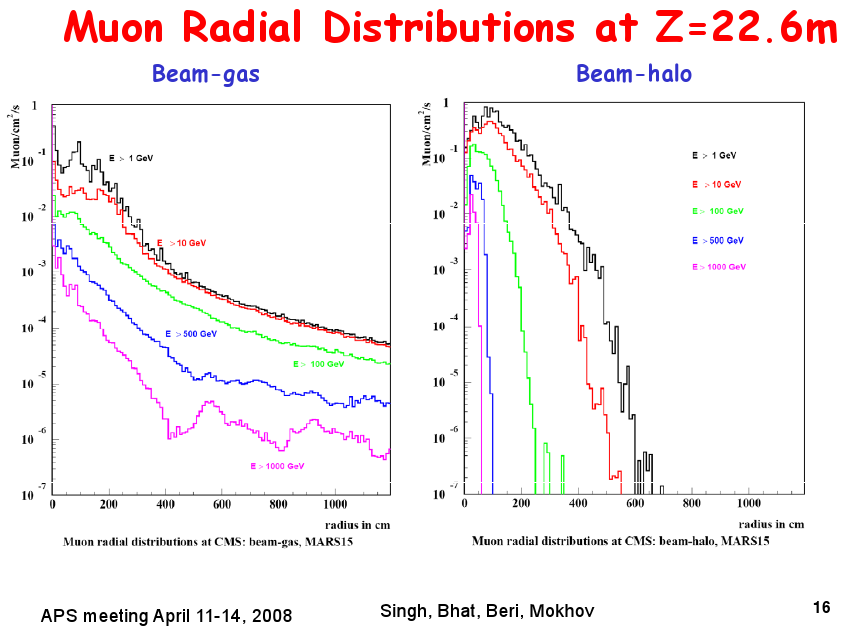
\includegraphics[width=\linewidth]{slide.png}

\tiny
\textcolor{blue}{\tt \underline{\href{http://indico.cern.ch/materialDisplay.py?contribId=0&materialId=slides&confId=30868}{http://indico.cern.ch/materialDisplay.py?contribId=0\&materialId=slides\&confId=30868}}}

Careful! Rates quoted above are for $10^{34}$!
\end{frame}

%% \section*{First section}
%% \begin{frame}
%% \begin{center}
%% \Huge \textcolor{blue}{First section}
%% \end{center}
%% \end{frame}

\begin{frame}
\frametitle{Implications}

\textcolor{darkblue}{``Beam-halo'' versus ``Beam-gas''?}
\begin{itemize}
\item We have not been making a distinction, but this is how I understand it:

\hfill 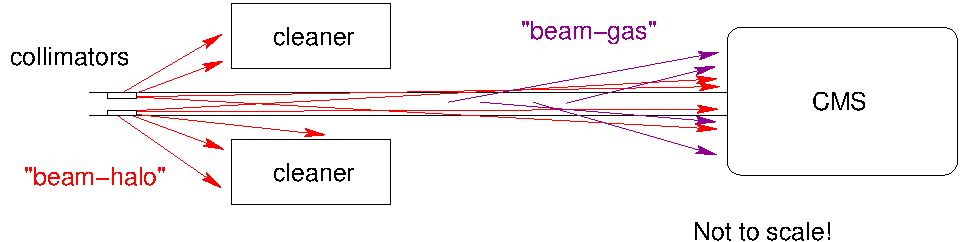
\includegraphics[width=0.8\linewidth]{diagram.pdf}
\end{itemize}

\textcolor{darkblue}{For alignment:}
\begin{itemize}
\item Inner ring may be covered by beam-halo, but only beam-gas provides high-momentum tracks
\end{itemize}

\vfill
\textcolor{darkblue}{For TeV-showering studies (Joe Gartner):}
\begin{itemize}
\item Only beam-gas will do
\end{itemize}

\vfill When single-beam/machine studies begin in June and we collect
CSC data, we should be most interested in days with bad vaccuum, rather
than days with narrow collimators

\label{numpages}
\end{frame}

\end{document}
